\documentclass{article}
\usepackage{caption}
\usepackage{subcaption}
\usepackage{amsmath}
\usepackage{amssymb}
\usepackage{mathtools}
\usepackage[margin=0.75in]{geometry}
\usepackage{fancyhdr}
\usepackage{xcolor}
\usepackage{tikz}
\usepackage[normalem]{ulem} % for strike through text
\setlength{\headheight}{0in}

\newcommand{\problemsep}{\leavevmode\\[0.05in] \rule[\baselineskip/4]{\textwidth}{1pt} \\[0.005in] \rule[\baselineskip]{\textwidth}{1pt}\vspace{-\baselineskip/2}\leavevmode\\[0.05in]}
\newcommand{\statementsep}{\leavevmode\\[0.005in] \rule[\baselineskip/4]{\textwidth}{0.4pt}\leavevmode\\[0.005in]}
\pagestyle{fancy}
\rhead{\today}
\lhead{Daniel Mortensen}
\chead{Homework 4}

\begin{document}
\noindent\underline{Problem 1}: Please sort all trees on $8$ vertices into homeomorphism classes.
\statementsep
The trees with $8$ vertices are given as \\
\begin{center}
\begin{tabular}{c |c | c | c | c | c | c | c | c |}
 & 1 & 2 & 3 & 4 & 5 & 6 & 7 & 8 \\ \hline
1 & 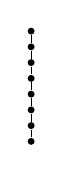
\begin{tikzpicture}[scale=0.05, every node/.style={circle, inner sep=0pt, minimum size=2.5pt, fill=black}, level distance=4cm, level/.style={sibling distance=8cm/#1}]
  \node(root){}
    child {node{}
    child {node{}
	child {node{}
	child {node{}
	child {node{}
	child {node{}
	child {node{}}}}}}}};
\end{tikzpicture} & 
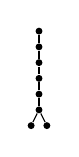
\begin{tikzpicture}[scale=0.05, every node/.style={circle, inner sep=0pt, minimum size=2.5pt, fill=black}, level distance=4cm, level 6/.style={sibling distance=4cm}]
  \node(root){}
    child {node{}
    child {node{}
	child {node{}
	child {node{}
	child {node{}
		child {node{}}
		child {node{}}}}}}};
\end{tikzpicture} &
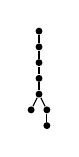
\begin{tikzpicture}[scale=0.05, every node/.style={circle, inner sep=0pt, minimum size=2.5pt, fill=black}, level distance=4cm, level 5/.style={sibling distance=4cm}]
  \node(root){}
    child {node{}
   	child {node{}
	child {node{}
	child {node{}
		child {node{}}
		child {node{}
			child {node{}}}}}}};
\end{tikzpicture} &
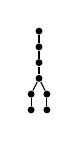
\begin{tikzpicture}[scale=0.05, every node/.style={circle, inner sep=0pt, minimum size=2.5pt, fill=black}, level distance=4cm, level 4/.style={sibling distance=4cm}]
  \node(root){}
    child {node{}
   	child {node{}
	child {node{}
		child {node{}
			child {node{}}}
		child {node{}
			child {node{}}}}}};
\end{tikzpicture} &
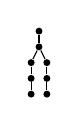
\begin{tikzpicture}[scale=0.05, every node/.style={circle, inner sep=0pt, minimum size=2.5pt, fill=black}, level distance=4cm, level 2/.style={sibling distance=4cm}]
  \node(root){}
    child {node{}
		child {node{}
			child {node{}
				child {node{}}}}
		child {node{}
			child {node{}
				child {node{}}}}};
\end{tikzpicture} &
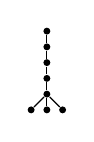
\begin{tikzpicture}[scale=0.05, every node/.style={circle, inner sep=0pt, minimum size=2.5pt, fill=black}, level distance=4cm, level/.style={sibling distance=4cm}]
  \node(root){}
    child {node{}
	child {node{}
	child {node{}
	child {node{}
		child {node{}}
		child {node{}}
		child {node{}}}}}};
\end{tikzpicture} &
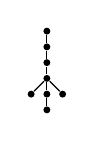
\begin{tikzpicture}[scale=0.05, every node/.style={circle, inner sep=0pt, minimum size=2.5pt, fill=black}, level distance=4cm, level 4/.style={sibling distance=4cm}]
  \node(root){}
    child {node{}
	child {node{}
	child {node{}
		child {node{}}
		child {node{}
			child {node{}}}
		child {node{}}}}};
\end{tikzpicture} &
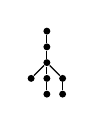
\begin{tikzpicture}[scale=0.05, every node/.style={circle, inner sep=0pt, minimum size=2.5pt, fill=black}, level distance=4cm, level 3/.style={sibling distance=4cm}]
  \node(root){}
    child {node{}
	child {node{}
		child {node{}}
		child {node{}
			child {node{}}}
		child {node{}
			child {node{}}}}};
\end{tikzpicture} \\ \hline
2 & 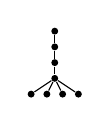
\begin{tikzpicture}[scale=0.05, every node/.style={circle, inner sep=0pt, minimum size=2.5pt, fill=black}, level distance=4cm, level 3/.style={sibling distance=4cm}]
  \node(root){}
    child {node{}
	child {node{}
	child {node{}
		child {node{}}
		child {node{}}
		child {node{}}
		child {node{}}}}};
\end{tikzpicture} &
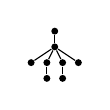
\begin{tikzpicture}[scale=0.05, every node/.style={circle, inner sep=0pt, minimum size=2.5pt, fill=black}, level distance=4cm, level/.style={sibling distance=8cm/#1}]
  \node(root){}
    child {node{}
		child {node{}}
		child {node{}
			child {node{}}}
		child {node{}
			child {node{}}}
		child {node{}}};
\end{tikzpicture} &
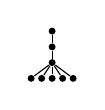
\begin{tikzpicture}[scale=0.05, every node/.style={circle, inner sep=0pt, minimum size=2.5pt, fill=black}, level distance=4cm, level/.style={sibling distance=8cm/#1}]
  \node(root){}
    child {node{}
	child {node{}
		child {node{}}
		child {node{}}
		child {node{}}
		child {node{}}
		child {node{}}}};
\end{tikzpicture} &
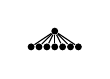
\begin{tikzpicture}[scale=0.05, every node/.style={circle, inner sep=0pt, minimum size=2.5pt, fill=black}, level distance=4cm, level/.style={sibling distance=2cm/#1}]
  \node(root){}
		child {node{}}
		child {node{}}
		child {node{}}
		child {node{}}
		child {node{}}
		child {node{}}
		child {node{}};
\end{tikzpicture} &
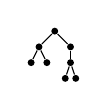
\begin{tikzpicture}[scale=0.05, every node/.style={circle, inner sep=0pt, minimum size=2.5pt, fill=black}, level distance=4cm, level/.style={sibling distance=8cm/#1}]
  \node(root){}
		child {node{}
			child {node{}}
			child {node{}}}
		child {node{}
			child {node{}
				child {node{}}
				child {node{}}}};
\end{tikzpicture} &
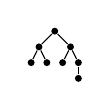
\begin{tikzpicture}[scale=0.05, every node/.style={circle, inner sep=0pt, minimum size=2.5pt, fill=black}, level distance=4cm, level/.style={sibling distance=8cm/#1}]
  \node(root){}
		child {node{}
			child {node{}}
			child {node{}}}
		child {node{}
			child {node{}}
			child {node{}
				child {node{}}}};
\end{tikzpicture} &
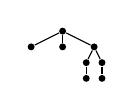
\begin{tikzpicture}[scale=0.05, every node/.style={circle, inner sep=0pt, minimum size=2.5pt, fill=black}, level distance=4cm, level/.style={sibling distance=8cm/#1}]
  \node(root){}
		child {node{}}
		child {node{}}
		child {node{}
			child {node{}
					child {node{}}}
			child {node{}
					child {node{}}}};
\end{tikzpicture} &
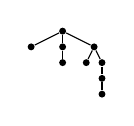
\begin{tikzpicture}[scale=0.05, every node/.style={circle, inner sep=0pt, minimum size=2.5pt, fill=black}, level distance=4cm, level/.style={sibling distance=8cm/#1}]
  \node(root){}
		child {node{}}
		child {node{}
			child {node{}}}
		child {node{}
			child {node{}}
			child {node{}
				child {node{}
					child {node{}}}}};
\end{tikzpicture} \\ \hline
3 & 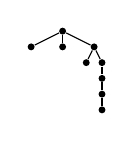
\begin{tikzpicture}[scale=0.05, every node/.style={circle, inner sep=0pt, minimum size=2.5pt, fill=black}, level distance=4cm, level/.style={sibling distance=8cm/#1}]
  \node(root){}
		child {node{}}
		child {node{}}
		child {node{}
			child {node{}}
			child {node{}
				child {node{}
					child {node{}
						child {node{}}}}}};
\end{tikzpicture} &
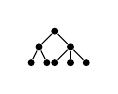
\begin{tikzpicture}[scale=0.05, every node/.style={circle, inner sep=0pt, minimum size=2.5pt, fill=black}, level distance=4cm, level/.style={sibling distance=8cm/#1}]
  \node(root){}
		child {node{}
			child {node{}}
			child {node{}}}
		child {node{}
			child {node{}}
			child {node{}}
			child {node{}}};
\end{tikzpicture} &
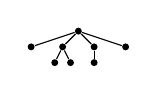
\begin{tikzpicture}[scale=0.05, every node/.style={circle, inner sep=0pt, minimum size=2.5pt, fill=black}, level distance=4cm, level/.style={sibling distance=8cm/#1}]
  \node(root){}
		child {node{}}
		child {node{}
			child{node{}}
			child{node{}}}
		child {node{}
				child {node{}}}
		child {node{}};
\end{tikzpicture} &
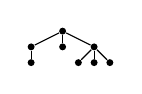
\begin{tikzpicture}[scale=0.05, every node/.style={circle, inner sep=0pt, minimum size=2.5pt, fill=black}, level distance=4cm, level/.style={sibling distance=8cm/#1}]
  \node(root){}
		child {node{}
			child {node{}}}
		child {node{}}
		child {node{}
			child {node{}}
			child {node{}}
			child {node{}}};
\end{tikzpicture} &
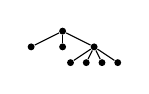
\begin{tikzpicture}[scale=0.05, every node/.style={circle, inner sep=0pt, minimum size=2.5pt, fill=black}, level distance=4cm, level/.style={sibling distance=8cm/#1}]
  \node(root){}
		child {node{}}
		child {node{}}
		child {node{}
			child {node{}}
			child {node{}}
			child {node{}}
			child {node{}}};
\end{tikzpicture} &
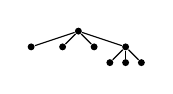
\begin{tikzpicture}[scale=0.05, every node/.style={circle, inner sep=0pt, minimum size=2.5pt, fill=black}, level distance=4cm, level/.style={sibling distance=8cm/#1}]
  \node(root){}
		child {node{}}
		child {node{}}
		child {node{}}
		child {node{}
			child {node{}}
			child {node{}}
			child {node{}}};
\end{tikzpicture}  &
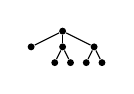
\begin{tikzpicture}[scale=0.05, every node/.style={circle, inner sep=0pt, minimum size=2.5pt, fill=black}, level distance=4cm, level/.style={sibling distance=8cm/#1}]
  \node(root){}
		child {node{}}
		child {node{}
			child {node{}}
			child {node{}}}
		child {node{}
			child {node{}}
			child {node{}}};
\end{tikzpicture} & 
\end{tabular}
\end{center}
and each homeomorphism class is given in the table below along with the index of each corresponding tree. \\
\begin{center}
\begin{tabular}{c | c | c | c}
	Homeomorphism Class & Tree Indices & Homeomorphism Class & Tree Indices \\ \hline
	
\begin{tikzpicture}[scale=0.05, every node/.style={circle, inner sep=0pt, minimum size=2.5pt, fill=black}, level distance=4cm, level/.style={sibling distance=8cm/#1}]
		\node(root){}
			child {node{}};
	\end{tikzpicture} & (1,1) &
	
\begin{tikzpicture}[scale=0.05, every node/.style={circle, inner sep=0pt, minimum size=2.5pt, fill=black}, level distance=4cm, level/.style={sibling distance=8cm/#1}]
		\node(root){}
			child {node{}
				child {node{}}
				child {node{}}};
	\end{tikzpicture} & (1,2), (1,3), (1,4), (1,5) \\ \hline
		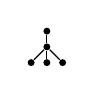
\begin{tikzpicture}[scale=0.05, every node/.style={circle, inner sep=0pt, minimum size=2.5pt, fill=black}, level distance=4cm, level/.style={sibling distance=8cm/#1}]
		\node(root){}
			child {node{}
				child {node{}}
				child {node{}}
				child {node{}}};
	\end{tikzpicture} & (1,6), (1,7), (1,8) &
	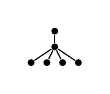
\begin{tikzpicture}[scale=0.05, every node/.style={circle, inner sep=0pt, minimum size=2.5pt, fill=black}, level distance=4cm, level/.style={sibling distance=8cm/#1}]
		\node(root){}
			child {node{}
				child {node{}}
				child {node{}}
				child {node{}}
				child {node{}}};
	\end{tikzpicture} & (2,1), (2,2) \\ \hline
 	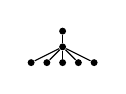
\begin{tikzpicture}[scale=0.05, every node/.style={circle, inner sep=0pt, minimum size=2.5pt, fill=black}, level distance=4cm, level/.style={sibling distance=8cm/#1}]
		\node(root){}
			child {node{}
				child {node{}}
				child {node{}}
				child {node{}}
				child {node{}}
				child {node{}}};
	\end{tikzpicture} & (2,3) &
	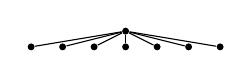
\begin{tikzpicture}[scale=0.05, every node/.style={circle, inner sep=0pt, minimum size=2.5pt, fill=black}, level distance=4cm, level/.style={sibling distance=8cm/#1}]
		\node(root){}
			child {node{}}
			child {node{}}
			child {node{}}
			child {node{}}
			child {node{}}
			child {node{}}
			child {node{}};
	\end{tikzpicture} & (2,4) \\ \hline
	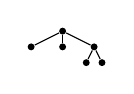
\begin{tikzpicture}[scale=0.05, every node/.style={circle, inner sep=0pt, minimum size=2.5pt, fill=black}, level distance=4cm, level/.style={sibling distance=8cm/#1}]
		\node(root){}
				child {node{}}
				child {node{}}
				child {node{}
					child {node{}}
					child {node{}}};
	\end{tikzpicture} & (2,5), (2,6), (2,7), (2,8), (3,1), (3,2)&
	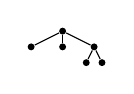
\begin{tikzpicture}[scale=0.05, every node/.style={circle, inner sep=0pt, minimum size=2.5pt, fill=black}, level distance=4cm, level/.style={sibling distance=8cm/#1}]
		\node(root){}
				child {node{}}
				child {node{}}
				child {node{}
					child {node{}}
					child {node{}}};
	\end{tikzpicture} & (2,7), (2,8), (3,1) \textcolor{red}{start here}\\ \hline
	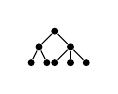
\begin{tikzpicture}[scale=0.05, every node/.style={circle, inner sep=0pt, minimum size=2.5pt, fill=black}, level distance=4cm, level/.style={sibling distance=8cm/#1}]
		\node(root){}
				child {node{}
					child {node{}}
					child {node{}}}
				child {node{}
					child {node{}}
					child {node{}}
					child {node{}}};
	\end{tikzpicture} & (3,2) &
	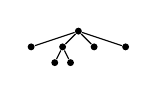
\begin{tikzpicture}[scale=0.05, every node/.style={circle, inner sep=0pt, minimum size=2.5pt, fill=black}, level distance=4cm, level/.style={sibling distance=8cm/#1}]
		\node(root){}
				child {node{}}
				child {node{}
					child {node{}}
					child {node{}}}
				child {node{}}
				child {node{}};
	\end{tikzpicture} & (3,2)

\end{tabular}
\end{center}
\problemsep
\noindent\underline{Problem 2}: Show that the graph $G$ (defined later) is not planar in two ways: (1) Use 
Kuratowski's Theorem, and (2) use the Euler identity $n-e+f=2$.
\textsf{Notation:} For $n \in \mathbb{N}$, $[n] = \{1,2,3,\dots, n\}$, and $[0] =\O$.
Define $G = (V,E)$ as follows.  Let $V = \{\mbox{$2$-sets of } [5]\}$, with 
vertices $x$ and $y$ adjacent if and only if $x \cap y = \O$.
\statementsep
\textcolor{red}{insert text her} 
\problemsep
\noindent\underline{Problem 3:} Please prove that no pair of the directed graphs in the figure below are 
isomorphic.
\begin{center}
    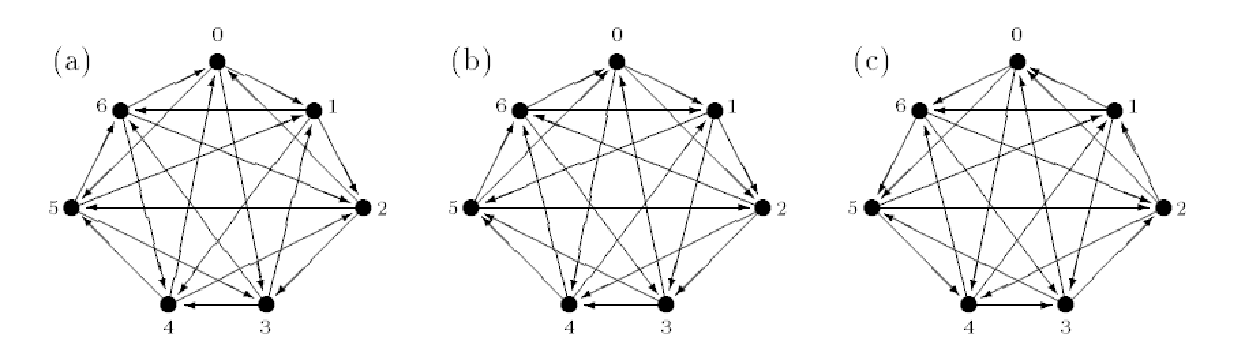
\includegraphics[scale=0.75]{media/reg7Ts.pdf}
\end{center}
\statementsep
\textcolor{red}{insert solution here}
\end{document}
